%!TEX root = vaisagh_thesis.tex

\chapter{Modeling Event Identification Behavior in Agent Based Simulations Of Crowds}
\label{chapter:PreEvacuationBehavior}


Ideally, when a fire starts a fire alarm goes off, all occupants hear this alarm and use the nearest safe exit to leave the building. However, this is hardly the norm. In many cases, occupants are desensitized from hearing false alarms and often do not start to evacuate until they are completely sure that egress is necessary. On January 19, 2000, a fire in Boland Hall in Seton Hall University killed three students because they had ignored the fire alarms assuming they were false~\cite{Berry:2000us}. This uncertainty about the authenticity of the first sign of danger isn't an isolated incident~\cite{Graham:2000vl,Proulx:2001we,Proulx:1995wq,Proulx:2003tc,Purser:2001ts,Ramachandran:1990wj,Sime:1995uu,Tong:1985wn}. This delay in reaction time of evacuees are likely to ruin existing plans for egress if it is not taken into consideration. Hence, when studying the behavior of evacuees, it is necessary to study and understand their actions from the time at which the fire started right up until the point where the last person evacuated~\cite{Tong:1985wn}.



As discussed in Chapters~\ref{chapter:LiteratureReview} and~\ref{chapter:IBEVAC}, pre-evacuation uncertainty and investigation are features of human behavior during egress that are rarely considered in existing models. To recap, \emph{pre-evacuation} refers to the period of time that elapses after the start of the fire alarm before the person starts evacuating. While some models~\cite{Tsai:2011tz} do have a simplified model of pre-evacuation behavior, they fail to model it in enough detail to enable their extension to more general cases. For example, a fire alarm could have different effects based on the clarity and believability of the alarm~\cite{Kobes:2009jx,Paulsen:1984ti}. This variability is hard to simulate in existing models of pre-evacuation behavior. Also, during an evacuation people exchange event and environment related information with others. Evacuees are unlikely to follow every message that they receive blindly. There is a variability in the \emph{trust} in messages received that can have different effects on egress. This is rarely considered in existing models.


In this chapter, we present a model for simulating pre-evacuation behavior and event identification in agent based simulations of crowds~\footnote{This model was presented as a poster and short paper at the Pedestrian and Evacuation Dynamics Conference in 2012~\cite{Viswanathan:2012vt}.}. In the model, the evacuees identify and process information in terms of event cues which exist throughout the environment. Section~\ref{PreEvac:LitRev} first explores some of the existing work that motivates the need to model pre-evacuation behavior. Following this, Section~\ref{PreEvac:EventIdentification} explains the proposed model and, finally, Section~\ref{PreEvac:Results} illustrates through experimentation the usefulness of this model, the importance of modeling pre-evacuation behavior and having a communication model.



\section{Related Work}
\label{PreEvac:LitRev}


As discussed in Section~\ref{LiteratureReview:CurrentUnderstanding}, there are a lot of conflicting theories on how humans behave in emergencies and why they behave as they do. However, there are also certain parts of human nature that are generally accepted to be true, such as the constant search for information~\cite{Proulx:2003tc,Tong:1985wn,Ozel:2001tn,Sime:1983uy}. This section first summarizes the existing knowledge of human behavior during egress with special emphasis on pre-evacuation behavior. Following this, some existing models of pre-evacuation behavior and communication are presented.

\subsection{On modeling Pre-evacuation behavior}
\label{PreEvac:PreEvacuationBehavior}

Several studies of human behavior during emergency egress~\cite{Kuligowski:2005tt,Ozel:2001tn,Proulx:2007ul}, have shown that an evacuee's first reaction after realizing that there is an unusual situation is to investigate and gather more information about the situation. Evacuation starts only once the need for evacuation is established. \emph{Cues} are the key to understanding this transition from realization to investigation and, eventually, to evacuation.

Cues are certain changes in the environment that indicate that something is wrong or different from normal~\cite{Sime:1983uy}.
They come in different forms. Fire and smoke are the typical and most effective cues for an evacuation. Fire alarms and people running about or instructing to escape are also cues. According to Sime~\cite{Sime:1983uy}, there are three kinds of cues:
\begin{itemize}
\item Ambiguous Cues: E.g. Hearing noises or shouting, or seeing someone run.
\item Verbal Cues: E.g. Instructions from a companion, announcement from the stage.
\item Unambiguous Cues: E.g. Seeing smoke or fire, or seeing someone run with a fire extinguisher.
\end{itemize}


According to some researchers~\cite{Ramachandran:1990wj,Proulx:2007ul}, an ambiguous cue by itself does not cause a person to initiate investigation. Rather, the cue has to persist for a period of time before investigation begins and results in the finding of an unambiguous cue. Interestingly, according to Tong and Canter~\cite{Tong:1985wn}, even unambiguous cues don't result in people immediately exiting the building, rather it initiates a complicated process consisting of information searching and affiliation.

The effect of cues and the evacuee's reaction to it depends on many factors. The identity of an individual's primary group and its proximity and availability determines the reaction of a person to a cue~\cite{Sime:1983uy}. The classic study presented in~\cite{Latane:1969wm}, participants where placed in a room with smoke. The experiment showed that when alone, 75 percent of the subjects reported the smoke. In the presence of two non-reacting others only 10 percent of the subjects reported the smoke during the experimental period.

Various studies~\cite{Proulx:2003tc,Proulx:2001we,Paulsen:1984ti,Sandberg:1997tw,Cocking:2008vv,Tong:1985wn} emphasize the importance of the location and the person's role in the significance of cues. As an example, a fire alarm at home is more likely to cause a person to act than a fire alarm at their office, which will most likely be considered a false alarm. People's societal role determines their training and responsibility and thus their alertness to cues and the preparedness for reacting to it.

Their groups, location and environment aren't the only factors that influence people's behavior during evacuation. There are also a lot of \emph{intrinsic factors} that influence how people react to fires. What these factors are and how influential they are have always been a matter of much debate. Over the years there have been several surveys~\cite{Tong:1985wn,Sandberg:1997tw,Kuligowski:2009un} that discuss these intrinsic factors.

Andr\'{e}e and Eriksson's report~\cite{Andree:2008td} even had a cross cultural study that compared the evacuation behavior of Swedish students against the behavior of Australian students. Except for grouping behavior they found hardly any significant differences in the behavior during evacuations. Kobes et al., in their survey~\cite{Kobes:2009jx}, compared some studies of evacuation behavior from the USA, Great Britain and Australia and commented on them being ``identical in their essence''. Some factors like age and gender were found to not significantly affect pre-evacuation behavior. A person's social role is one of the commonly accepted factors that influence evacuation behavior~\cite{Sandberg:1997tw,Kobes:2009jx,Paulsen:1984ti}. Factors like the person's experience with fires, training, disabilities, familiarity with the environment, etc.\ are accepted to have a great influence on pre-evacuation behavior.

Close to a hundred different studies on human behavior in fires were used by Kuligowski~\cite{Kuligowski:2009un} to make a compilation of the factors that influence egress and more specifically pre-evacuation behavior. In this article, she suggests that the period that we term as \emph{pre-evacuation} itself consists of two phases. Phase 1 is called \emph{perception}; The idea being that just because a cue exists, does not imply that everyone perceives it. The Table~\ref{tab:Cues} lists some factors that can affect this perception of a person and whether these factors increase or decrease the chance of the person perceiving the abnormality in the situation.

Kuligowski calls the next phase \emph{interpretation}. During this phase, the person searches for more information to verify whether a fire has actually started and if it actually poses a threat that needs to be handled. Many studies~\cite{Ozel:2001tn,Proulx:2007ul} have confirmed the importance of this phase, though sometimes they are known by different names. In~\cite{Ozel:2001tn} this phase is called \emph{unconflicted inertia} to indicate how the person either continues what he's doing or tries to finish of his activity without actually beginning to evacuate. In~\cite{Tong:1985wn}, this phase is called \emph{investigation} to indicate the search for information that enables the interpretation of the system. Regardless of what it is called, this phase consists of two parts:
\begin{inparaenum}
\item defining the situation as a fire and
\item defining the risk that the situation poses.
\end{inparaenum}


Kuligowski categorized the factors that influence these phases into two types: occupant based factors~(which are equivalent to the intrinsic factors mentioned earlier) and cue based factors. These factors and their effects are shown in Table~\ref{tab:Cues}. Increases/Decreases signifies a cues effect on that particular phase. Also, cue based factors, do not simply consist of events, but also their nature and features.


% Requires the booktabs if the memoir class is not being used
\begin{table}[htbp]
\centering
\begin{threeparttable}[b]
\topcaption{Factors affecting Evacuation Behavior. The list of factors and their influences as presented in Kuligowski's survey~\cite{Kuligowski:2009un}} % requires the topcapt package
\begin{tabular}{m{6.3cm} c >{\centering\arraybackslash}m{2.8cm} >{\centering\arraybackslash}m{2.8cm}} % Column formatting, @{} suppresses leading/trailing space
\toprule
Factors & Perception  & 2a: Definition of the Situation as a Fire & 2b: Definition of the Risk to Self/Others\\

\midrule
\multicolumn {4}{l}{{\bf Occupant-based pre-event factors}}\\
\midrule
Has experience with fires    & Increases  & Increases &  Increases\\
Has knowledge of fire/ training & Increases  & Increases &  Increases\\
Habituation with environment   & Decreases  & ---\tnote{1}    &  --- \\
Has knowledge of routes     &   ---   &  ---    & Decreases\\
Has frequent experience with false alarms & ---  & Decreases &  ---\\
Has a feeling of security in the building & ---  & Decreases &  ---\\
Has perceptual disability   & Decreases  & --- &  ---\\
Is older adult        & Decreases  & --- &  Increases\\
Is woman           & Increases  & --- &  Increases\\
Speaks the same language as others & Increases  & --- &  ---\\
Has frequent interaction with family & Increases  & --- &  ---\\
\midrule
\multicolumn {4}{l}{{\bf Occupant-based event factors}}\\
\midrule
Has a higher stress/ anxiety level  & Decreases & --- & --- \\
Perceives a time pressure & Decreases & Decreases & Increases \\
Presence of others~(especially loved ones) & Decreases & --- & Increases \\
Proximity to fire / Visual Access  & Increases & --- & --- \\
Sleeping & Decreases & ---& ---\\
A higher number of behavioral processes(>1) & --- & Increases & --- \\
Defines situation as a fire & -- & N/A & --- \\
\midrule
\multicolumn {4}{l}{{\bf Cue-based factors}}\\
\midrule
A higher number of cues & Mixed\tnote{2} & Increases & Increases \\
Consistent cues & --- & Increases & Increases \\
Unambiguous cues & --- & Increases & --- \\
Social cues~(others' actions) that are consistent with an understanding of a fire situation & --- & Increases & Increases \\
Official source & Increases & Increases &---\\
Familiar source & --- & Increases &--- \\
A higher dose of toxic gases & --- & Decreases & --- \\
Extreme/ dense cues & Decreases & --- & Increases \\
Visual/ audible cues & Increases & --- & --- \\
Risk Information & --- & Increases & --- \\
\bottomrule
\end{tabular}
\begin{tablenotes}
\item[1]{Areas where no research is found is marked by ---}
\item[2]{Research conflicted on the direction of influence of this factor}
\end{tablenotes}
\label{tab:Cues}
\end{threeparttable}
\end{table}



One of the factors that encourage the programmatic implementation of cue based factors is the fact that the effect of a cue can be explained to be caused by the nature and characteristics of the cue rather than the specific cue. In other words, each cue can be described in terms of its ambiguity, consistency with other cues and its source and it is this description that determines the effect of the cue.


\subsection{Existing models}
\label{PreEvac:ExistingModels}

There are very few existing models that take the pre-evacuation period into consideration. Pires~\cite{Pires:2005gs}  modeled the pre-evacuation decision making of an individual using a simple Bayesian Belief Network~(BBN).

Fran{\c c}a et al.~\cite{Franca:2009wq} created a simulation model of the development of panic behavior during emergency egress. This model implemented the hysterical belief theory~\cite{Torres:2010tj} and modeled how panic first develops and then evacuation happens. It also had a basic communication system through which agents exchanged mood information (which is a key factor in the development of panic) by using the grid based environment as a medium for communicating messages. Despite pre-evacuation behavior being modeled in some detail, it is not possible to extend this model to replicate the heterogeneity in people's reaction to cues.

ESCAPES~\cite{Tsai:2011tz} is a fairly recent model that takes into account some factors like the spread of knowledge, fear and emotion between the different evacuees. These factors are used to create a simplistic model of pre-evacuation behavior. Effectively though, only the \emph{perception} part of pre-evacuation behavior is modeled. This means that  once an agent perceives a cue i.e. another agent running, the perceiving agent immediately starts to evacuate.

The event identification and communication model proposed in this chapter have been influenced by these models but is unique in the way that the diversity of cues and their effects can be considered and more importantly in how both the perception and investigation phase can be modeled within this framework.

% \section{The IBEVAC Model}
% \label{IBEVAC}


% \begin{figure}[!tb]
% \centering
% 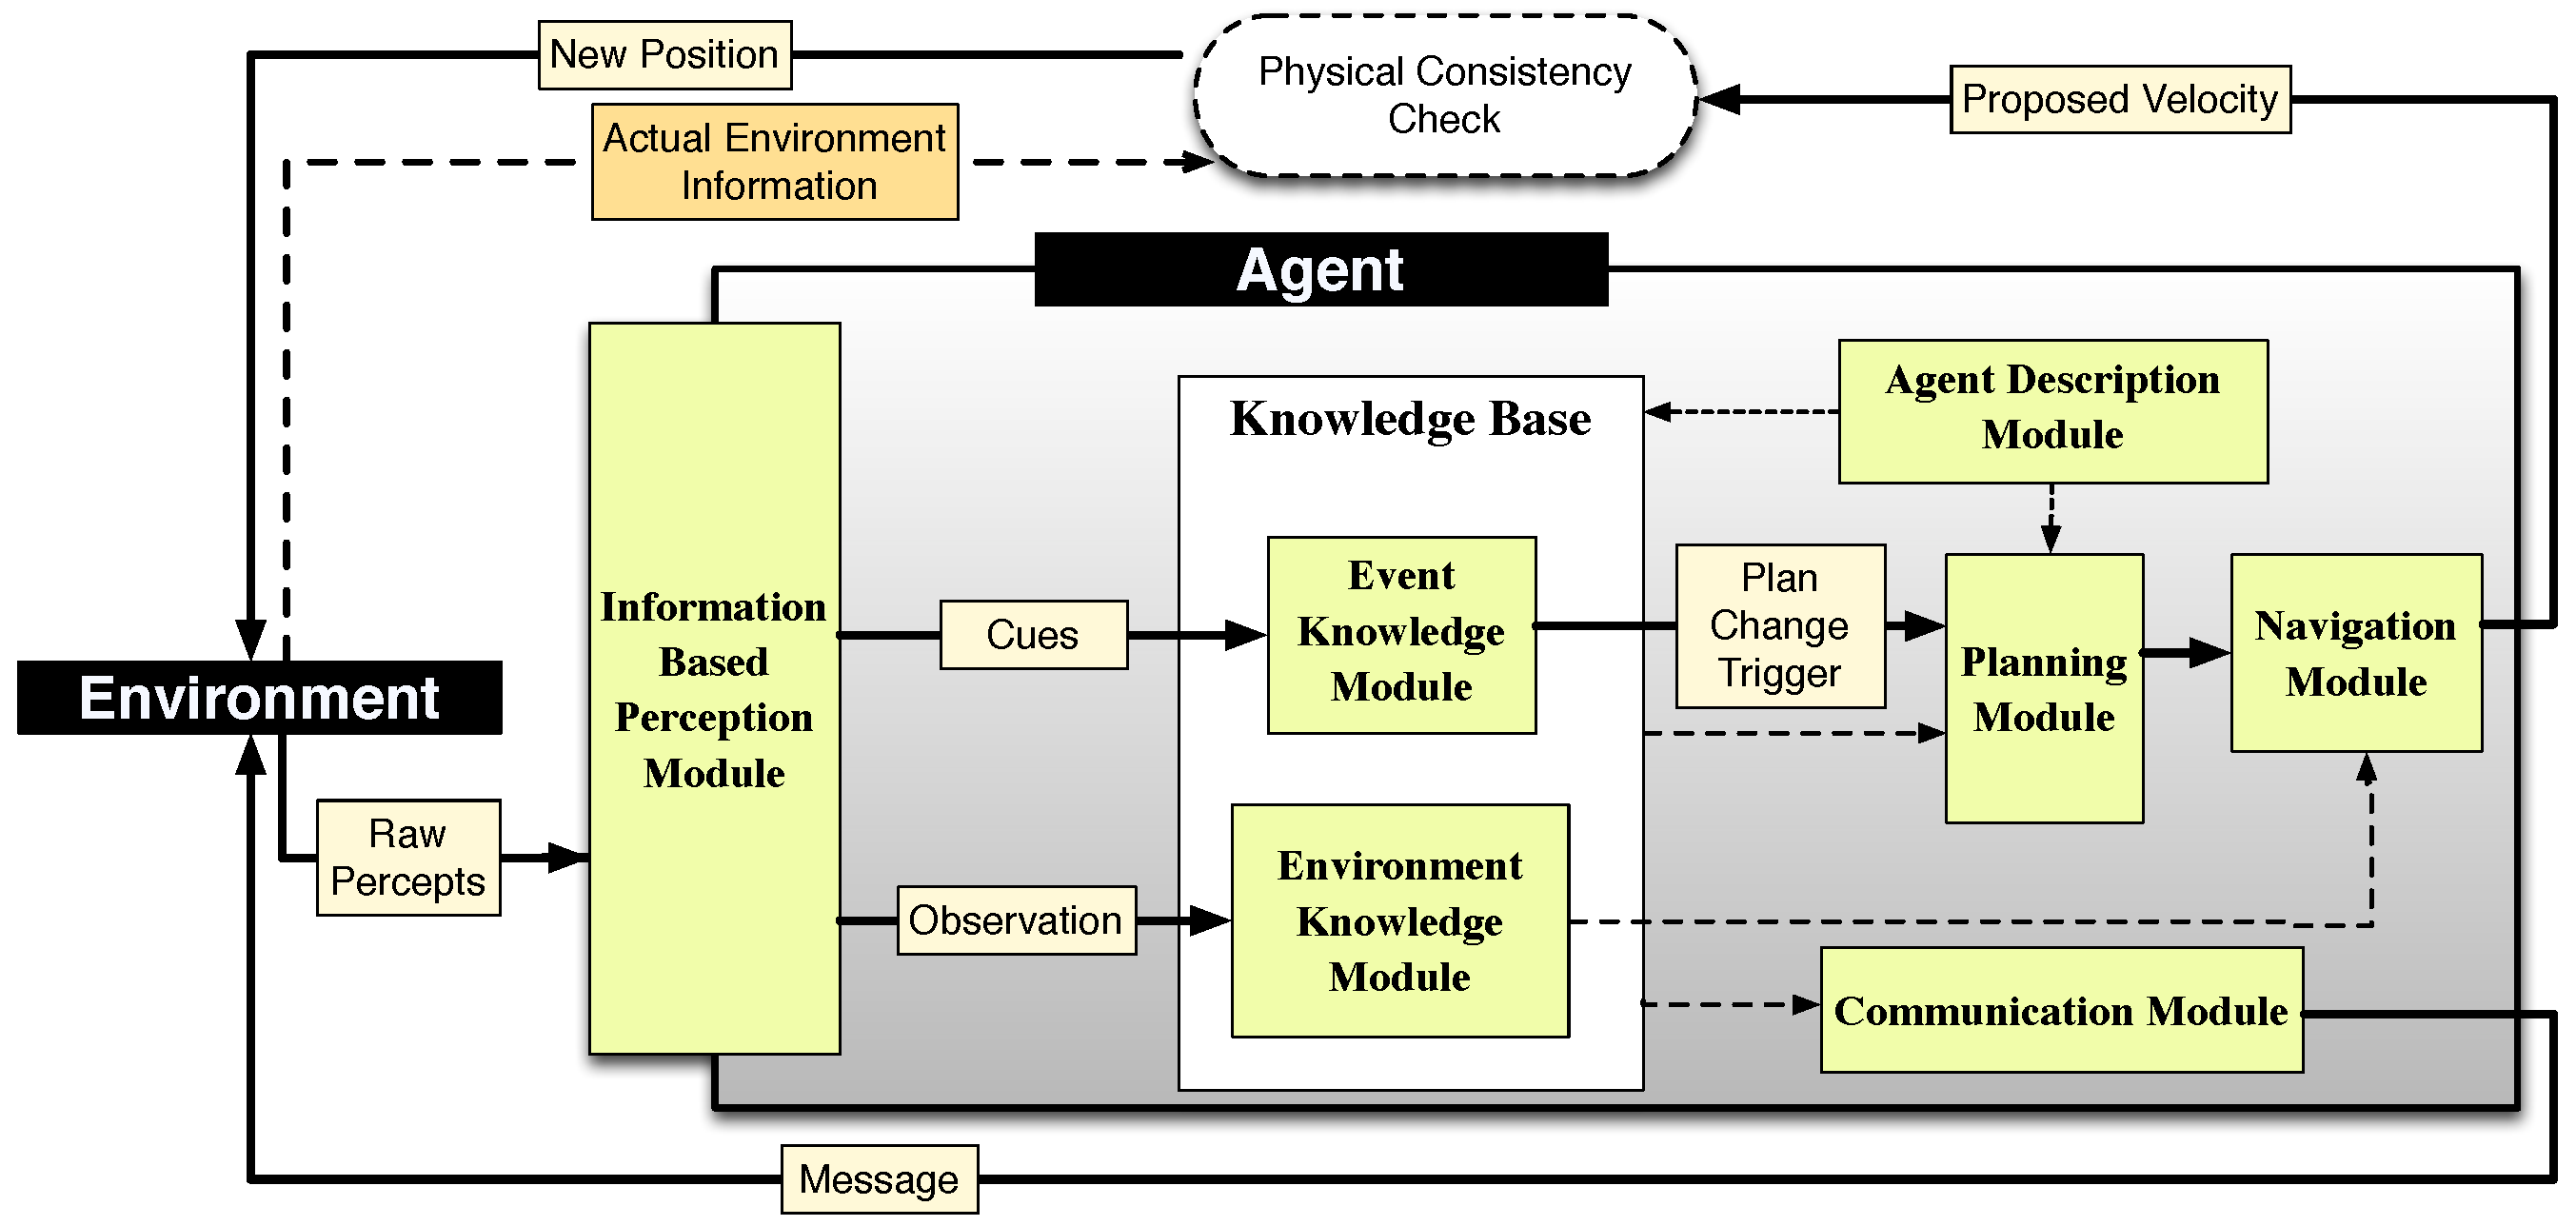
\includegraphics[height=1.9in]{SimplifiedAgentArchitecture}
% \caption[The Agent Architecture]{An illustrated representation of the IBEVAC agent architecture}
% \label{fig:AgentArchitecture}
% \end{figure}

% This section gives an overview of the modular IBEVAC agent architecture. Figure~\ref{fig:AgentArchitecture} shows this architecture. There are many objects or actions that an agent can sense or observe in the environment. We call these \emph{raw percepts}. According to their sources, they can be classified as \emph{observations} from the environment and \emph{messages} from other agents. The Information Based Perception~(IBP) Module is the only gateway through which the agent receives information from the environment. This module is explained in more detail in~\cite{Viswanathan:ut}. The IBP Module passes a percept to the Knowledge Base.

% The \emph{Environment Knowledge Module} stores a representation of the layout of the environment that is formed as a result of the observations of the agent. Information regarding accessibility of links is also stored. As a detailed discussion of this module is beyond the scope of this paper, all agents are assumed to have complete knowledge of the layout. However, agents can learn about inaccessible links only through direct observation or through messages from other agents. The {\em Event Knowledge Module} is the focus of research in this paper. It stores the agent's beliefs about the current state of the environment. Cue perception alters these beliefs and triggers a state change in the agent which is then handled by the Planning Module. This Module is explained in more detail in section~\ref{EventIdentification}.

% The intrinsic characteristics of the agent like the agent's size, speed, mass and social role are stored in the {\em Agent Description Module (ADM)}. It is also responsible for determining the strategies and actions taken by the Planning Module and in determining the effects of the cues on the Event Knowledge Module (Section~\ref{EventIdentification}). The {\em Planning Module} stores the current state of the agent i.e. whether it is exploring, milling or escaping and creates a plan of action for the agent as a set of goals. Each goal is a location that is passed to the Navigation Module.

\section{A Bucket Based Model of Event Identification}
\label{PreEvac:EventIdentification}

% First explain how cues are modeled
Section~\ref{PreEvac:PreEvacuationBehavior} discussed how ambiguity, source and consistency of the cue~\cite{Kuligowski:2005tt,Sime:1983uy,Tong:1985wn} are the key factors in determining the effect of a cue. This is the fundamental idea used in the proposed model. Each object or event that is to be perceived as a cue implements a \emph{Cue interface} which ensures that each cue can be explained in terms of these three factors. Each cue is located at a particular location in the environment and is sensed by agents when within their perception range. Thus when an event or an action of significance occurs at some location a cue is created at that location.


Once perceived, these cues are processed by the agent's \emph{Event Knowledge System} which manages the information from cues. The  module has two \emph{buckets} of information: one corresponding to \emph{investigation} and the second corresponding to \emph{egress}. When a cue is perceived, a certain amount of information is added to the respective bucket(s) based on the ambiguity level, consistency and source of the cue.  For each bucket, a \emph{threshold} is initially fixed  based on the intrinsic characteristics of the agent. When the amount of information in a bucket overflows the threshold the agent changes state/phase and changes it's goal to proceed towards a new goal based on the behavior model that is used. For the purpose of the experiments in this chapter, three kinds of goals (or behaviors) are chosen by the agent's planning system: normal behavior where the goal is the center of the \emph{home} room of the agent; \emph{milling} behavior where the agent gathers with other agents at the nearest \emph{corridor} (See Figure~\ref{fig:layout}); and \emph{evacuation} where the agent heads towards the nearest exit.


There are two sets of values here which have been mentioned: bucket thresholds and the amount of information that a cue contributes. As mentioned earlier, each cue is characterized by its consistency, source and ambiguity. The effect of consistency is modeled with the help of a boolean variable that says whether it indicates a need for egress or not. Cues that indicate a need to egress add information to buckets while cues that do not, remove information from it. Thus if an inconsistent set of cues are observed at a given time, less or maybe even no information might be added to each bucket.

The amount of information that is added or removed depends on the ambiguity and source of the cue. The key value in the \emph{bucket model} is the ambiguity of the cue. Each cue has an ambiguity value that is represented as a decimal value in the range $[0,1]$. Since each cue adds information to the \emph{investigation} and \emph{egress} buckets there are two information values associated with each ambiguity level of a cue corresponding to each respective bucket.

In theory, the amount of information added by a cue can be any decreasing function of the ambiguity of the cue. For simplicity, we assume that it is a linear function with the value added by a cue of ambiguity $\alpha$ to the bucket $\beta$ being given by:
\begin{equation}
	\mu_{\beta} (\alpha) =
    \begin{cases}
        +\infty & \mbox{ if } \alpha < \alpha^{min}_{\beta} \\
        {\tau}{\left[\frac{(\alpha^{max}_{\beta}-\alpha)* t^{max}_{\beta}}{\alpha^{max}_{\beta} - \alpha^{min}_{\beta}}\right]}^{-1} & \mbox{ if } \alpha^{max}_{\beta} \geq \alpha \geq \alpha^{min}_{\beta}\\
        0 & \mbox{ if } \alpha > \alpha^{max}_{\beta}
    \end{cases} \mbox{where } \beta \in \{\mbox{investigation, egress}\}
\end{equation}

Where $\tau$ is a constant equal to the egress bucket threshold value for a normal agent. $\tau$ is simply a constant that determines the slope of the curve and the range of $\mu$.  We arbitrarily choose a value $10,000$ for $\tau$ so that the rate of change of $\mu$ for every $0.1$ unit change in ambiguity is greater than $1$.

$t^{max}_{egress}$ is the maximum time taken by a person to start egress. Since there is no actual consensus on what this value should be, in the experiments here, this is taken as 600 seconds (10 minutes). $\alpha^{max}_{egress}$ refers to the maximum ambiguity level that has effect on the egress bucket which in this case is $0.9$ since we assume that cues more ambiguous than this do not add any information. This essentially helps us simulate those cues that only result in investigation even if they persist for a long time and never trigger evacuation itself. Correspondingly, $\alpha^{min}_{egress}$ refers to the ambiguity level at which egress begins immediately which we assume to be $0$.
% The formula above gives the relationship shown in figure~\ref{ambiguityInfoRelationship} between ambiguity level and time to start evacuation given a single cue of that ambiguity is perceived at each second.


A similar procedure is used to determine $\mu_{investigation}$. An ambiguity value of $1.0$ in this case represents a small amount of information, as opposed to no information in the case of the egress bucket. This is because even an unambiguous cue when perceived for long enough initiates investigation~\cite{Tong:1985wn}. An ambiguity value of $0.5$ corresponds to immediate start of investigation (TODO: investigation if this is even needed).
% Given this, $\mu_{investigation}$ can be calculated as:
% \begin{equation}
% 	\mu_{investigation} (\alpha) =
%     \begin{cases}
%         +\infty & \mbox{ if } \alpha < \alpha^{min}_{investigation} \\
%         {\tau}{\left[\frac{(\alpha^{max}_{investigation}-\alpha)* t^{max}_{investigation}}{\alpha^{max}_{investigation} - \alpha^{min}_{investigation}}\right]}^{-1} & \mbox{ if } \alpha^{max}_{investigation} \geq \alpha \geq \alpha^{min}_{investigation}\\
%         0 & \mbox{ if } \alpha > \alpha^{max}_{investigation}
%     \end{cases}
% \end{equation}
So, $\alpha^{max}_{investigation}$ and $\alpha^{min}_{investigation}$ are $1.0$ and $0.5$, respectively. $t^{max}_{investigation}$ which is the maximum time taken by an evacuee to begin investigation is arbitrarily fixed at half of $t^{max}_{egress}$ i.e. 300 seconds or 5 minutes since as with $t^{max}_{egress}$ we do not know what the actual value of this term is.

The value for threshold of each bucket is equal to $\tau$ for normal agents. For special agents, and to consider certain special scenarios and effects, we can simply choose a threshold that is lower than $\tau$ as will be demonstrated in the experiments in Sections~\ref{sec:experiment_3_informed_and_informing_agents} and~\ref{sec:experiment_4_modeling_the_effect_of_pre_evacuation_behavior}.


% Following this explain how messages contain message cues and additional information.
Communication is implemented as \emph{messages} sent from one agent to the other. Each message has a message cue and environment information. The message cue works just as other cues with it's own ambiguity level. Here the term ambiguity is used to refer to the trustworthiness of the source of the information. In the experiments in this chapter, the environment information that is passed is only about the inaccessible paths in the map.

In the experiments in this chapter, a simple cellular automata based fire model and a simple finite difference smoke model are executed. This creates fire and smoke cues at locations near the fire which spread as the simulation proceeds. The environment itself is made up of various rooms which are connected by links. Some rooms that link multiple rooms are marked as \emph{corridors} and are the gathering points for the agents when investigating. All agents are assumed to have complete spatial knowledge of the environment and initially start in their \emph{home} rooms. As soon as the fire starts, fire alarm cues are placed all over the environment. Agents react to these cues and mark observable pathways that are blocked as inaccessible in their Spatial Knowledge graph. All agents either escape or are killed at the end of the simulation.



% To recap the discussion in Chapter~\ref{chapter:IBEVAC}, the planning system of the agent on identifying a goal passes this goal to the Navigation System that proceeds through a three-level process to determine the preferred velocity of the agent. At the highest level, a logical path is determined in terms of rooms to be crossed from the agents current location to the goal. From this logical path, spatial way points or locations are extracted by the next level. The third and final level determines a possible collision free path to the farthest visible spatial waypoint. In the experiments in this chapter, A-Star is used for path planning and RVO2 is used for the motion planning system.


% Communication between agents is also modeled with agents being able to transmit messages within a fixed communication range.




\section{Results}
\label{PreEvac:Results}

% Outline what are the things that we expect to demonstrate
This section explains and illustrates the results produced by the experiments that were conducted to demonstrate the effect that cue perception and communication can have on egress. The experiments were conducted on the two floor office environment shown in Figure~\ref{fig:layout}. This was adapted from the World Trade Center in California.  Simulations were conducted with 200 agents randomly distributed all over the environment and data was collected after averaging over 100 replications of the simulation.

\begin{figure}[!tb]
\centering
\subfloat[Ground Floor]{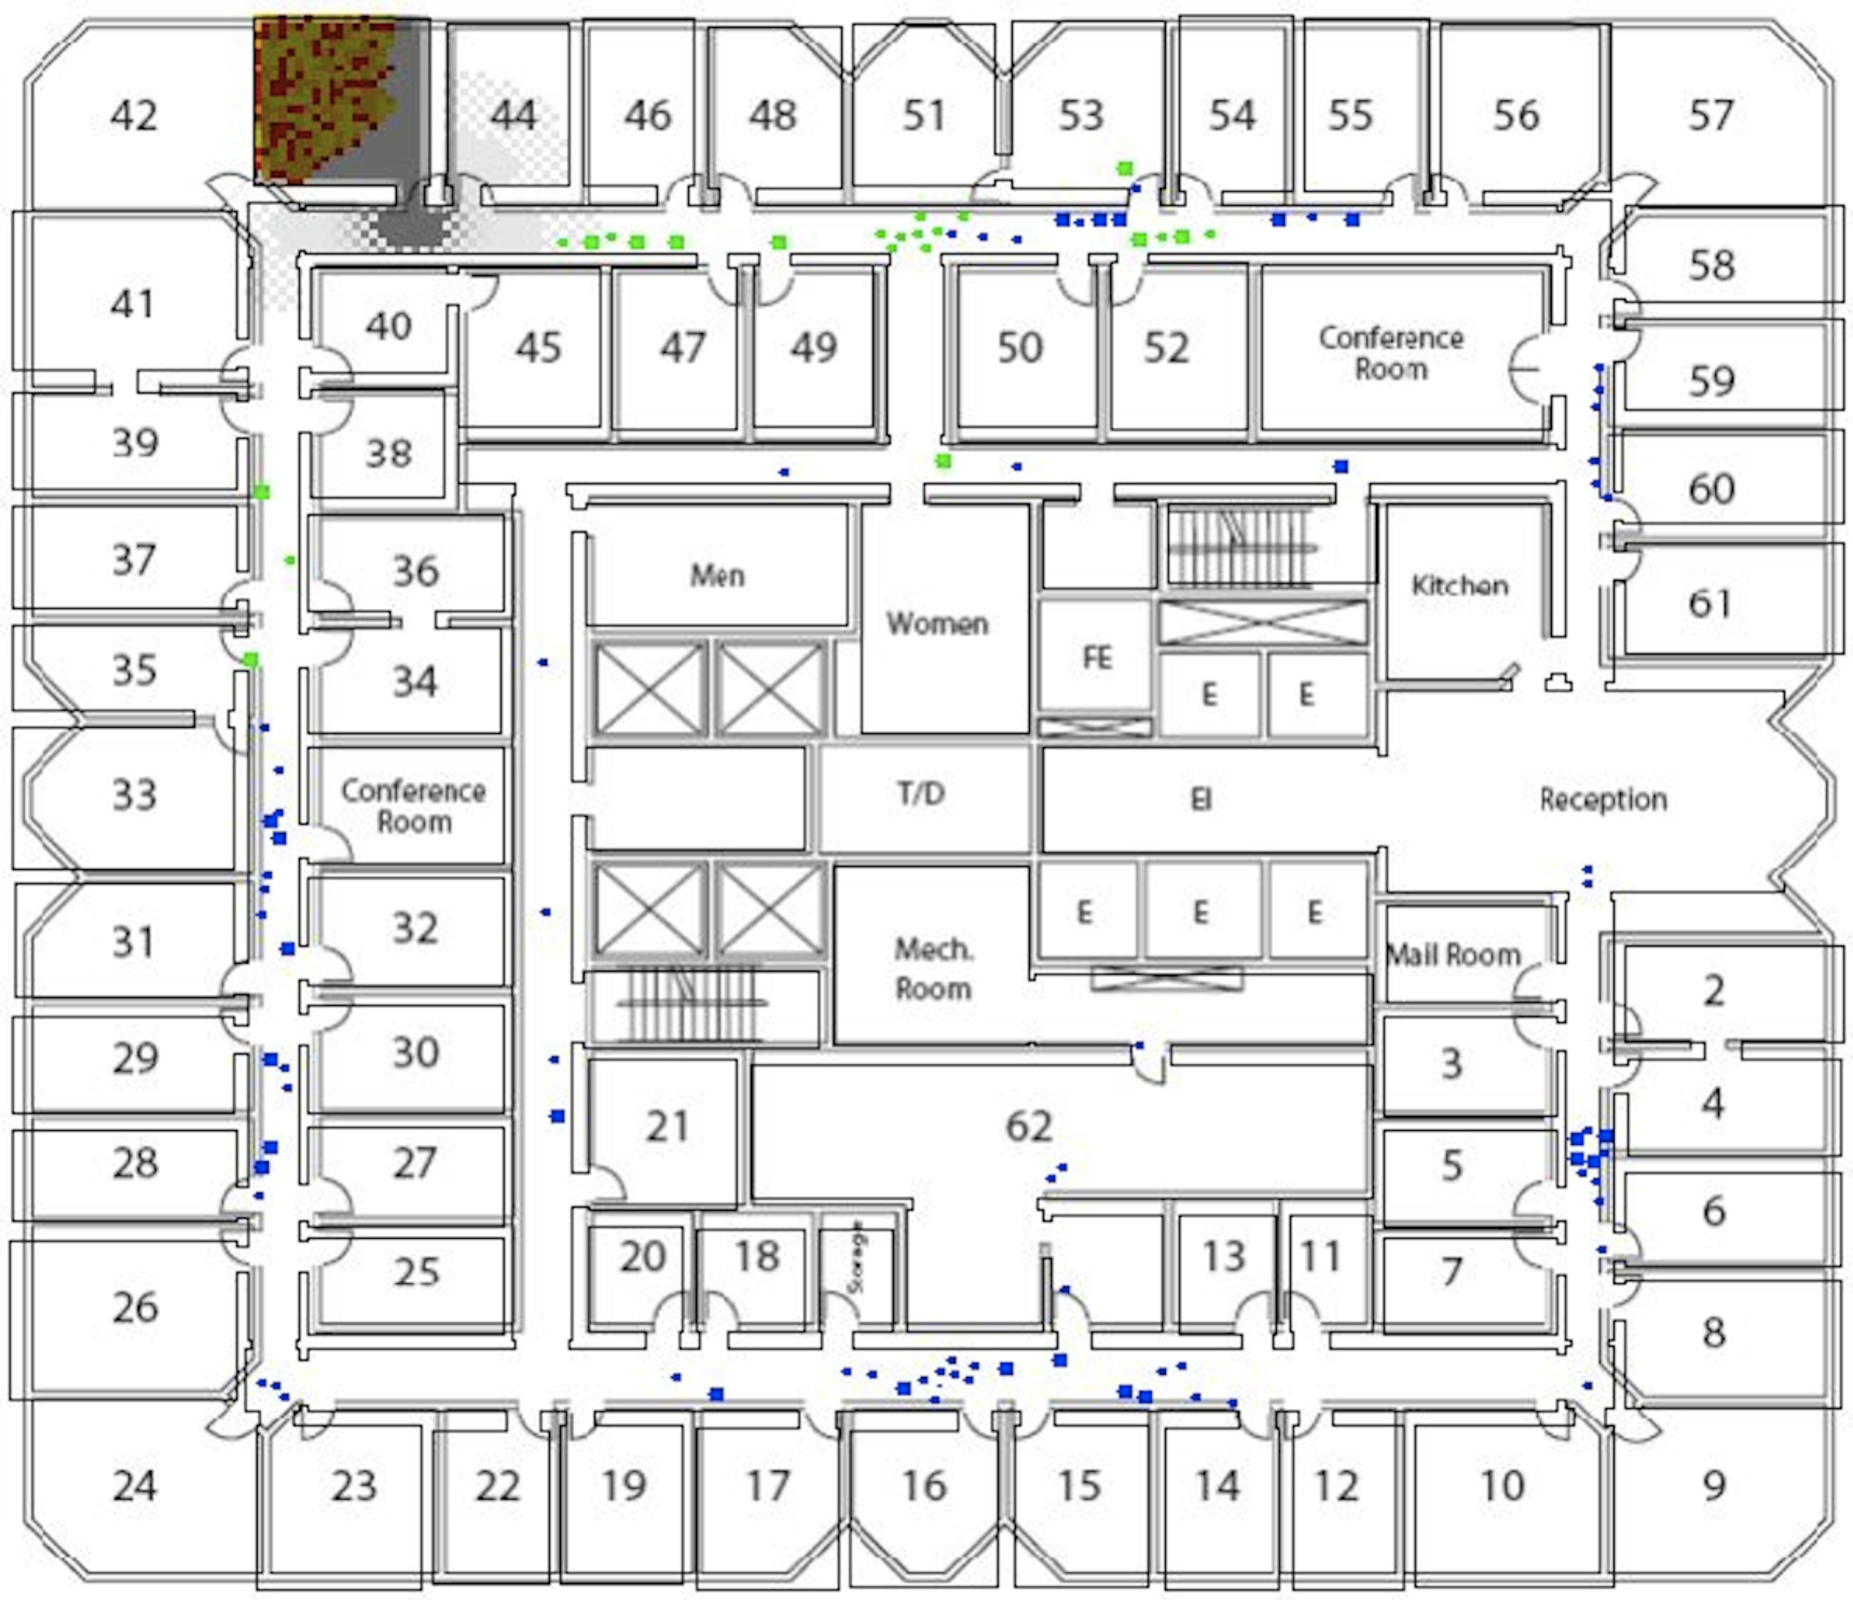
\includegraphics[width= 0.75\textwidth]{wtc-layout-level1}}
\\
\subfloat[Second Floor]{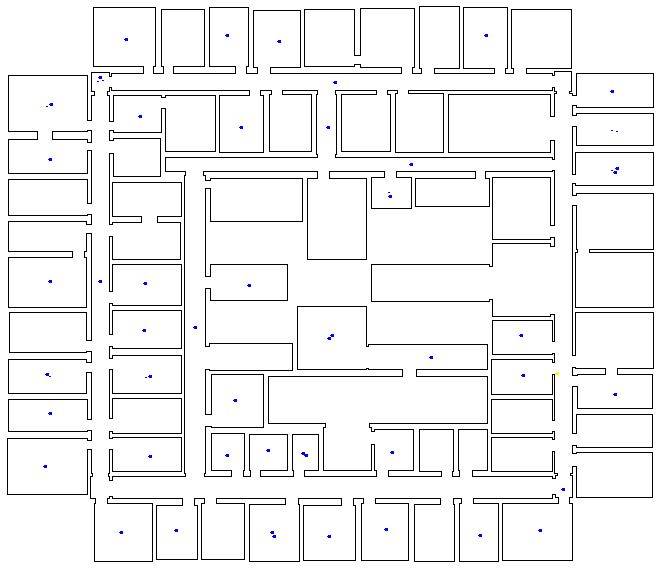
\includegraphics[width= 0.75\textwidth]{wtc-layout-level2.jpg}}
\caption[The Environment Layout]{First of two floors from World Trade Center, California. Fire in the figure is started in the corner room of the ground floor and generates smoke. Agents die immediately on contact with fire. Smoke depending on concentration initially slows and eventually kills agents. The longer rectangles are corridors connecting rooms and the open area on the right center of the ground floor is the exit. The red agents are those that are evacuating.}
\label{fig:layout}
% Change to my figure
\end{figure}

% Explain the layout of the environment, the settings and parameters

\subsection{Experiment 1: the effect of fire alarm ambiguity}
\label{PreEvac:experiment1}

In this experiment, the effect that fire alarm cue ambiguity has on egress was examined. It is assumed that the fire alarm can be heard clearly at every location on the map; so cues are placed in every room. A fire alarm with a simple ringing sound is much less clear and more ambiguous than a public announcement system that explicitly states that it is not a drill and gives real time updates about the situation.

To examine the effect of this difference in ambiguity, the experiment was repeated for different values of ambiguity (from $0.0$ - $1.0$). In this simulation, message cues are not simulated and the only other cues other than the Fire Alarm Cues are the Fire and Smoke Cues which are given ambiguities $0$ and $0.2$ respectively.

Figure~\ref{fig:SurvivalPlotDifferentRooms} shows the percentage of agents that escaped as a function of fire alarm ambiguity. As expected there is a significant drop in number of survivors as the ambiguity of the alarm increases. The experiments were conducted with the fire being started in different locations on the map (the locations chosen are shown in Figure~\ref{fig:RoomLayoutAnnotated}, to show to normalize the effect of the topography of the environment.

\begin{figure}[!tb]
	\centering
		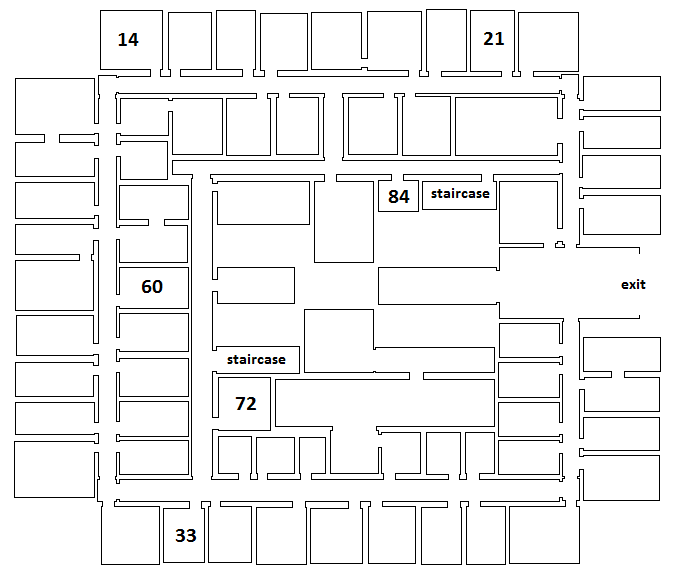
\includegraphics[width=\textwidth]{firealarm-room-marked}

	\caption{The layout of the ground floor with the relevant rooms, staircases and exit marked}
	\label{fig:RoomLayoutAnnotated}
\end{figure}
\begin{figure}[!tb]
	\centering
		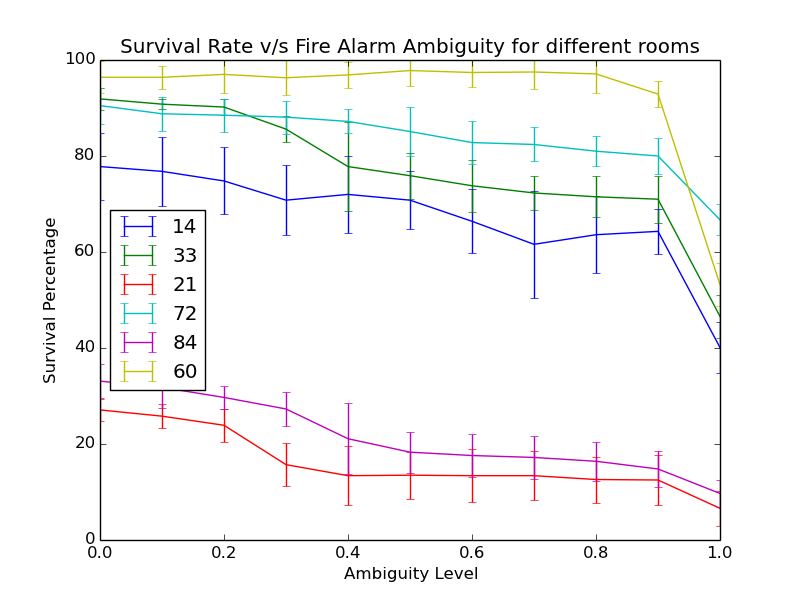
\includegraphics[width=\textwidth]{survivalPlotFireAlarmDifferentRooms}

	\caption{This figure shows the percentage of evacuees that survived as a function of the ambiguity with the fire being started in different rooms. While there are obvious inter room differences, it can be clearly seen that the more ambiguous an alarm, the lower the survival rate.}
	\label{fig:SurvivalPlotDifferentRooms}
\end{figure}

Regardless of room, the survival rate is quite high (generally above 80\%) with a clear and unambiguous fire alarm which prompts immediate evacuation from the agents while an unclear fire alarm which does not prompt immediate evacuation leads to much lower survival rates. While, the same pattern of higher ambiguity leading to reducing survival rate can be seen, there's a marked difference based on the room in which the fire is started.

The much lower survival rate for rooms 21 and 84 are because they are quite close to the exit and the exit gets closed relatively early in the simulation resulting in most agents failing to escape. The practically flat curve with very high survival rate for a fire starting in room 60 is because the room is far away from the exit with most agents having ample time to escape before any major exits or staircases are blocked. The curve for room 72 is similarly flat because the only major staircase that is blocked is the one that is further away from the fire. Also, since the smoke spreads to the second floor relatively quickly, the agents on the second floor start evacuating quickly as well.

In summary, it can be seen that the starting location of the fire does indeed have a significant effect on survival rate. It can also be clearly observed that a clear and unambiguous fire alarm can improve survival rates. The section has also demonstrated the the proposed model does model the effect that pre-evacuation delay can have on survival rates.



\subsection{Experiment 2:  modeling the effect of message propagation}
\label{PreEvac:experiment2}

In this experiment, the effect of message trustworthiness (ambiguity) is modeled. The fire alarm ambiguity is kept at $1.0$ to minimize its interference with the effect of message cues and the fire is started in room 14. Similar to experiment 1 the cue ambiguity is varied from $0.0$ to $1.0$. Figure~\ref{fig:MessageAmbiguityEffect} shows the time at which the last agent starts evacuating from the ground floor. Only the ground floor is taken since almost no agent on the higher floor start evacuating as they neither observe the fire nor get a message from other agents about the fire. It is interesting to note that even if all agents are completely trusted (ambiguity=0), the last agent still takes a long time ($\approx 1500$ seconds or 25 minutes after evacuation started) to start evacuating because it takes a long time for the information to propagate to it. The other effect that can be observed is that the rate of change becomes lower as the ambiguity increases.


\begin{figure}[!tb]
	\centering
		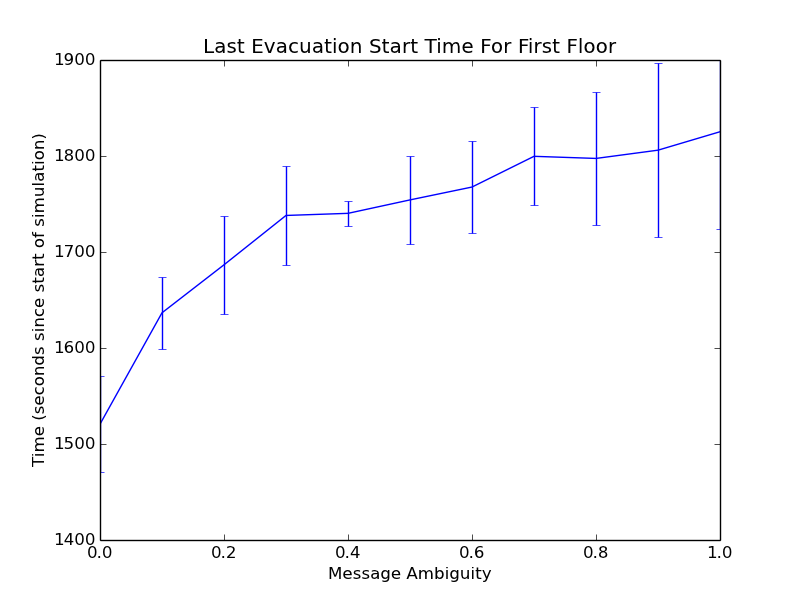
\includegraphics[width=\textwidth]{message_ambiguity_effect}
	\caption{This figure shows blah}
	\label{fig:SurvivalPlotDifferentRooms}
\end{figure}

\subsection{Experiment 3: Informed and Informing Agents} % (fold)
\label{sec:experiment_3_informed_and_informing_agents}

Assuming that it is possible to inform a certain number of occupants of a building about the urgent need to evacuate and these occupants inform others as they evacuate, an interesting question might be to examine how many people need to be informed for this strategy to be effective. To examine this we divide the set of agents into two groups: the normal agents and informed agents. The latter immediately start evacuating and broadcasting messages to other agents. The immediate evacuation can be modeled by settings the threshold of both buckets to zero. Message cues that have an informed agent as their source have an ambiguity of 0 indicating that these messages are completely trusted by other agents. The fire alarm ambiguity cue is again set to $1.0$ to minimize it's effect and, as in the previous experiment, the fire is started in room 14. Simulations were conducted with the proportion of informed agents varied from 5\% to 100\% of the 200 agents. The blue curve in Figure~\ref{fig:informed_vs_informing} shows the results of this experiment. Simulations showed that with just 15\% agents being informed the survival rate increased from 18.8\% to 55.5\%, an almost three fold increase. To isolate the effect of these informed agents propagating information, the red curve in the same figure shows the effect of these agents only being \emph{informed} agents that evacuate immediately without \emph{informing} other agents. The importance of these evacuating agents broadcasting the information they know is highlighted by the almost 30\% difference in survival rates that are observed when 15-60\% of the agents are informed.

\begin{figure}[!tb]
    \begin{center}
        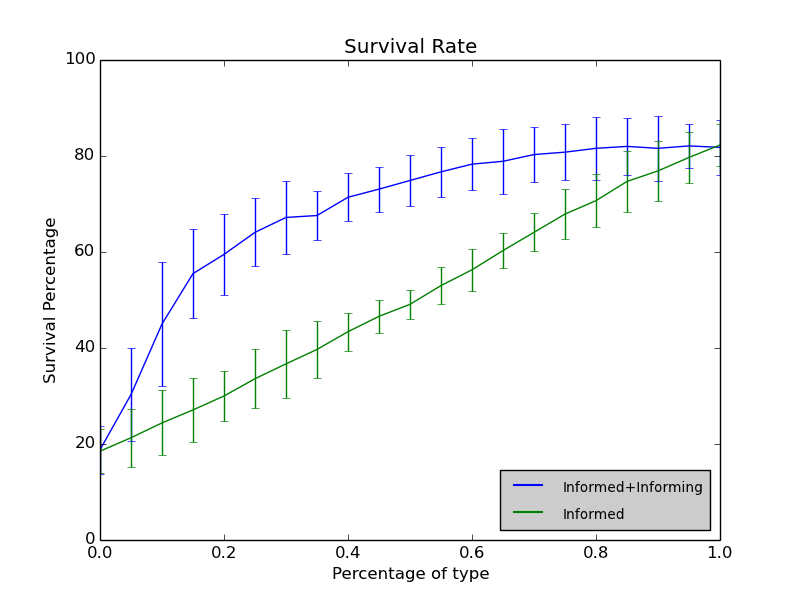
\includegraphics[width=\textwidth]{informed_vs_informing}
    \end{center}
    \caption{Figure showing informed vs informing}
    \label{fig:informed_vs_informing}
\end{figure}

% section experiment_3_informed_and_informing_agents (end)

\subsection{Experiment 4: is milling important?} % (fold)
\label{sec:experiment_4_modeling_the_effect_of_pre_evacuation_behavior}

The milling effect of people gathering in a common location to investigate and confirm the need to evacuate has been reported by interviewers of victims and is also one of the main features of the evacuation behavior modeled in the chapter. However, it is also a feature that is generally ignored in most models. Even in the rare cases that do consider pre-evacuation behavior, the \"pre evacuation behavior\" that is modeled is merely a delay in evacuation. In this section, the importance of modeling milling behavior is demonstrated.

\begin{figure}[!tb]
    \centering
        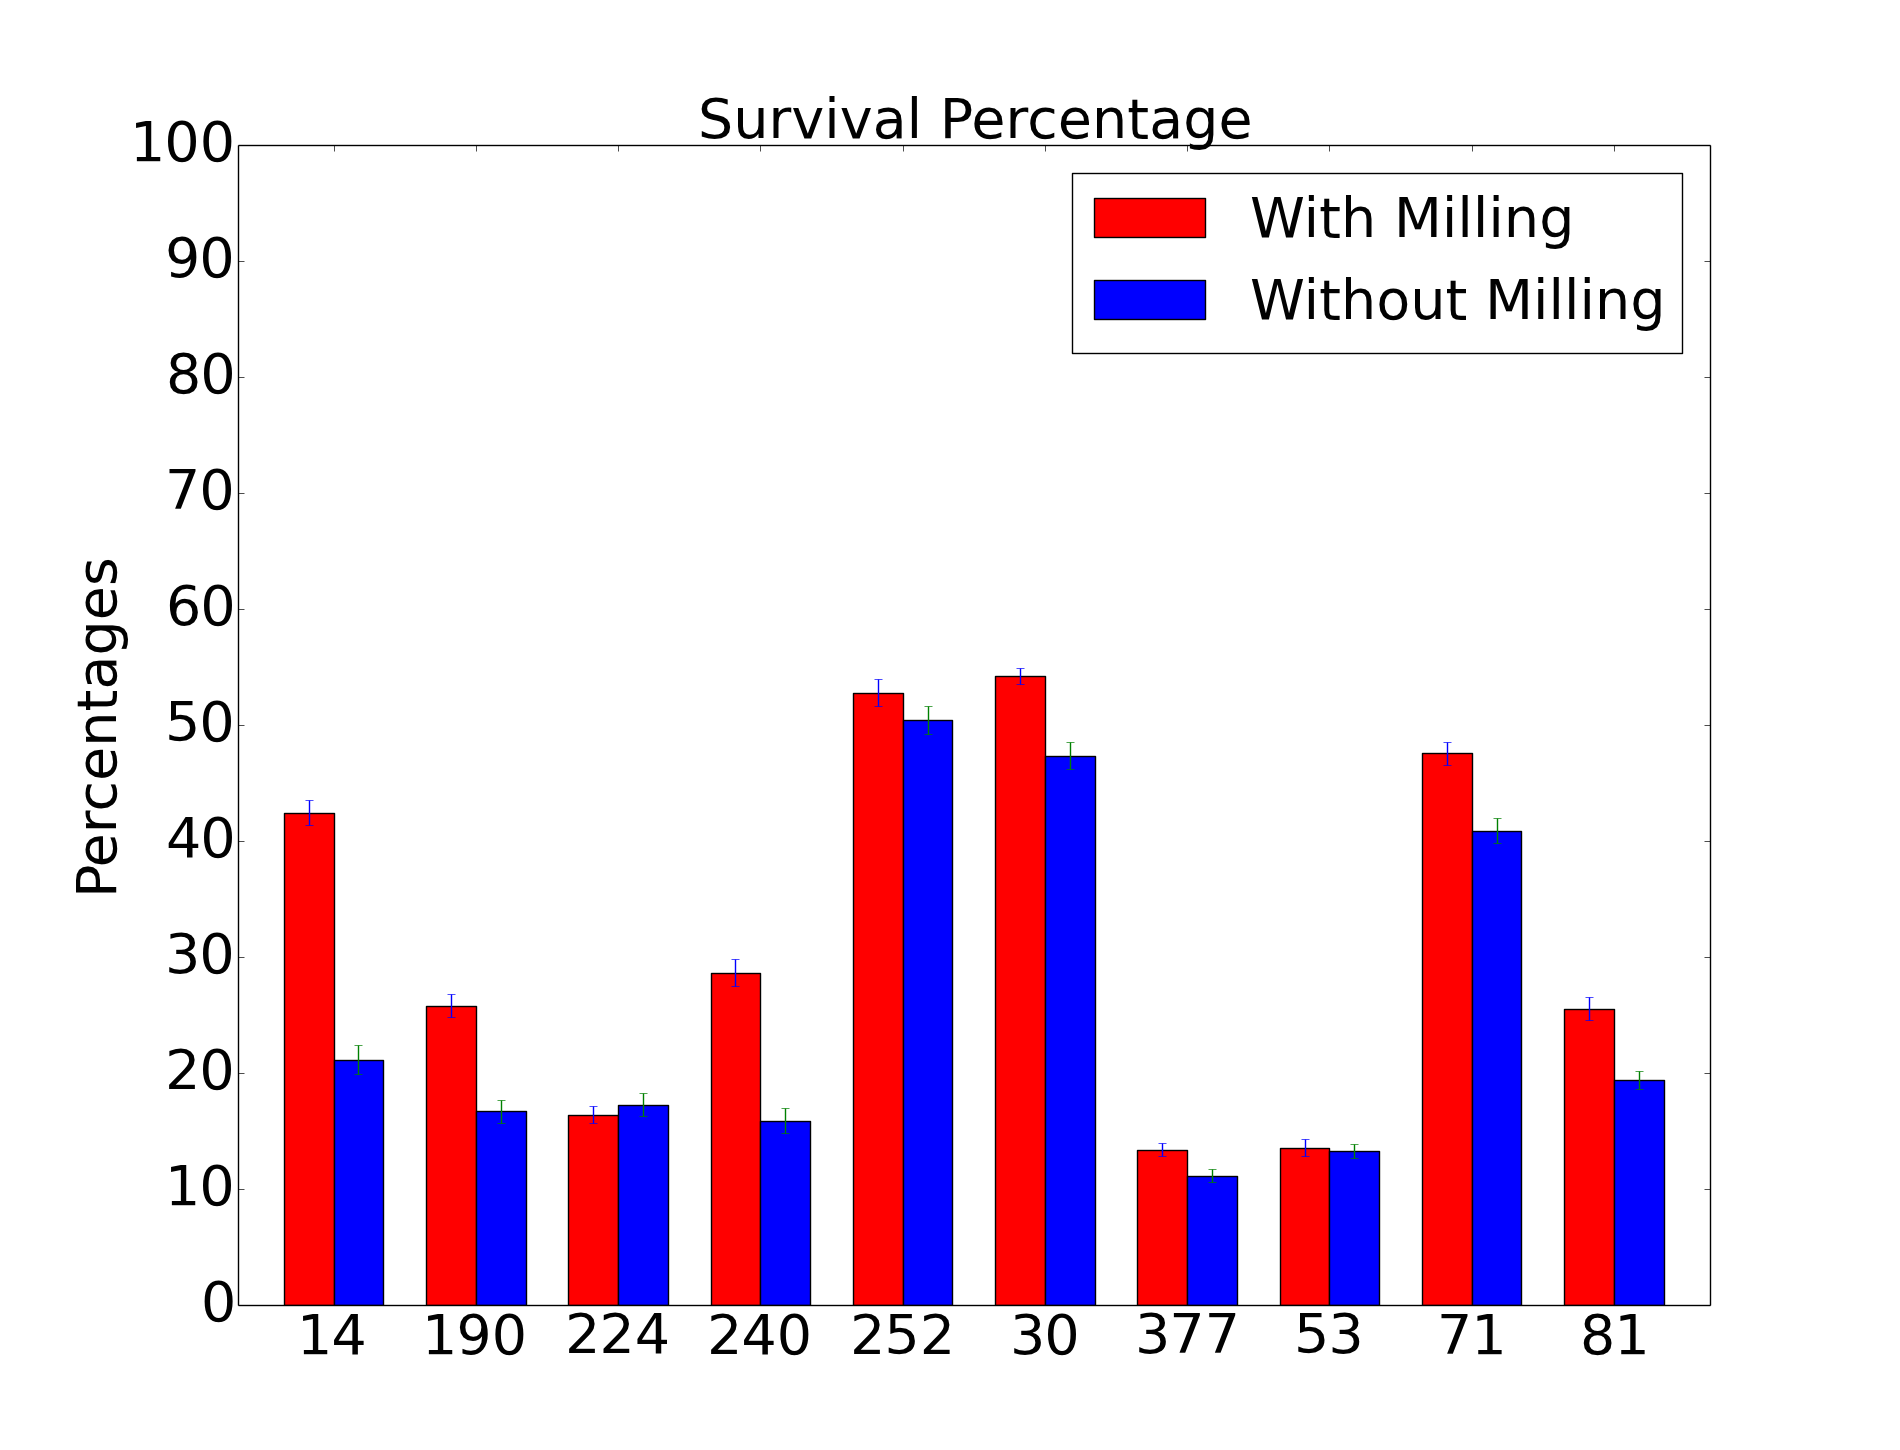
\includegraphics[width=\textwidth]{millingSurvivalPlot}

    \caption{Figure showing the effect of milling on survival rate}
    \label{fig:MillingSurvivalPlot}
\end{figure}
For this experiment, a new kind of agent that has an investigation threshold of positive infinity but an egress threshold of $\tau$ is modeled. These agents will start evacuating before their investigation bucket overflows. To test the hypothesis that milling behavior has a significant on evacuation characteristics, we compare these agents against the original agents with both their investigation and egress thresholds fixed at $\tau$. Since both agents have the same threshold for the egress bucket they will both start evacuating at the same time and the normal evacuation characteristics are identical. The importance and usefulness of milling is highlighted in the situation where evacuees communicate with each other. Figure~\ref{fig:MillingSurvivalPlot} compares the survival rates with milling against the situation where there is only delayed evacuation. As with experiment 2 (Section~\ref{PreEvac:experiment2}) we only consider the ground floor agents since fire alarm ambiguity is fixed at $1.0$. The figure clearly shows that if there is at least a certain amount of trust between agents then milling does indeed improve survival rates. This difference is much more clearly illustrated when we plot the average time at which the last agent starts evacuating in both situations shown in figure~\ref{fig:MillingLastPerson}.

\begin{figure}[!tb]
    \centering
        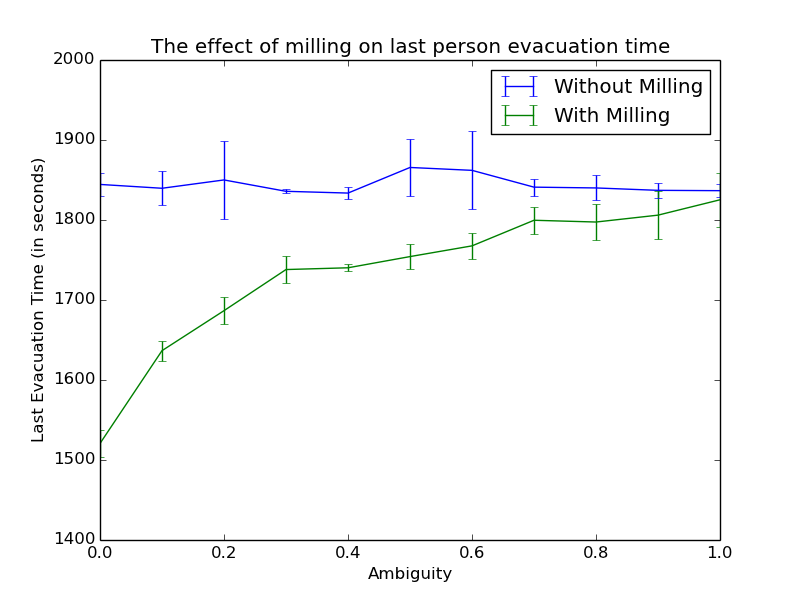
\includegraphics[width=\textwidth]{lastPersonMilling}
    \caption{Figure showing the average time at which last agent starts evacuating}
    \label{fig:MillingLastPerson}
\end{figure}

% section experiment_4_modeling_the_effect_of_pre_evacuation_behavior (end)
\section{Conclusion and Future Work}
\label{PreEvac:ConclusionAndFutureWork}

This chapter began with a discussion of the need to model pre-evacuation behavior. A novel cue modeling and perception system which enables the detailed modeling of pre-evacuation behavior was then described. It was demonstrated through simulation than modelling pre-evacuation behavior and the effect of ambiguity of perceived cues can have significant effects on evacuation efficiency. It was also shown that modelling how not all messages are trusted can also have a significant effect on evacuation dynamics.

In the future, it might be possible to make use of game based experiments like the one proposed in Chapter~\ref{chapter:SpatialKnowledgeChapter} can be used for understanding more about cues, and their effect and pre-evacuation behavior in general. It would also be interesting to try and model all, or at least most of the parameters defined by Kuligowski within the proposed framework.

In the simulations in this chapter it was assumed that each agent had complete knowledge of the environment, at least in terms of every room and how to get to each room. This is almost never the situation in the real world and to improve the efficacy of simulations it is necessary to model this partial knowledge. However, our current understanding of how people explore a partially known environment and how their knowledge develops over time are both very limited. The next chapter presents a game based methodology for studying this.
